\documentclass{article}

\usepackage{graphicx}

\usepackage{geometry}
\geometry{	a4paper,	total={210mm,297mm},	left=0mm,	top=10mm,	right=0mm,}
%\usepackage{blindtext}
%\usepackage[paperheight=10.75in,paperwidth=8.25in,margin=1in,heightrounded,showframe]{geometry}

\begin{document}

\begin{figure}[!tbp]
  \centering
  \begin{minipage}[b]{0.3\textwidth}
    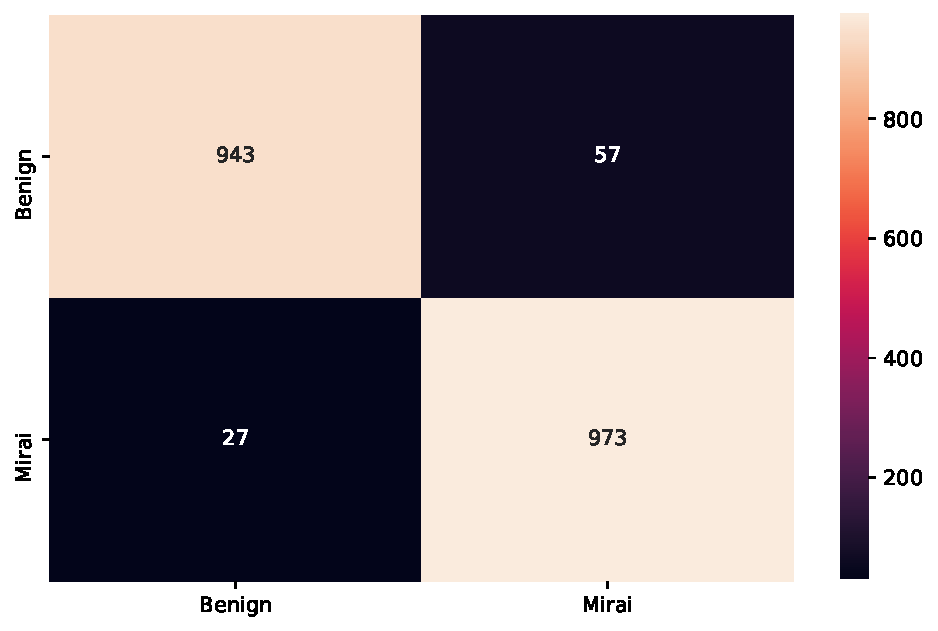
\includegraphics[width=\textwidth]{1.pdf}
    \caption{Flower one.}
  \end{minipage}
  %\hfill
  \begin{minipage}[b]{0.3\textwidth}
    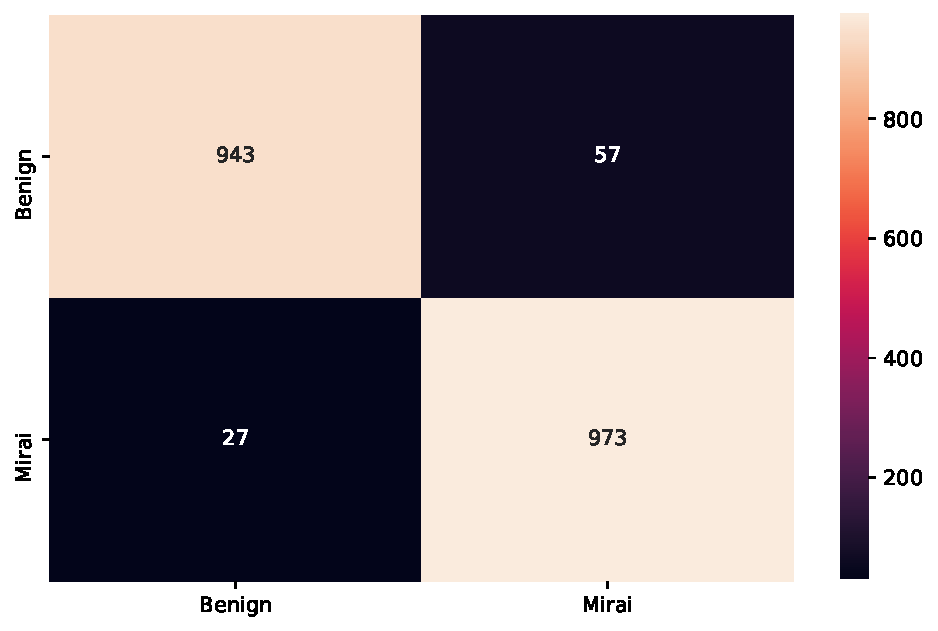
\includegraphics[width=\textwidth]{1.pdf}
    \caption{Flower two.}
  \end{minipage}


\end{figure}



\begin{figure}[htp]
	
	\centering
	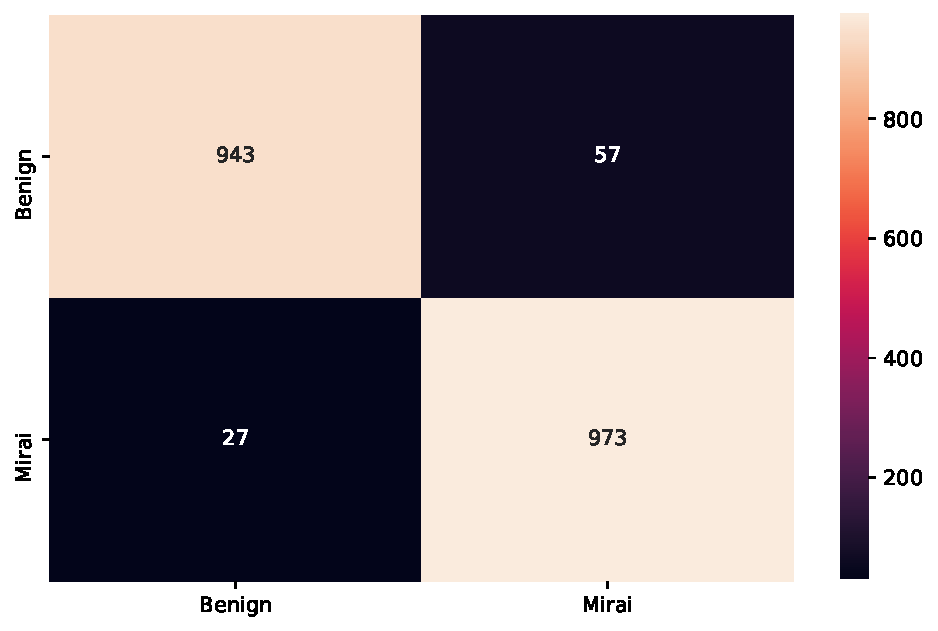
\includegraphics[width=.15\textwidth]{1.pdf}
	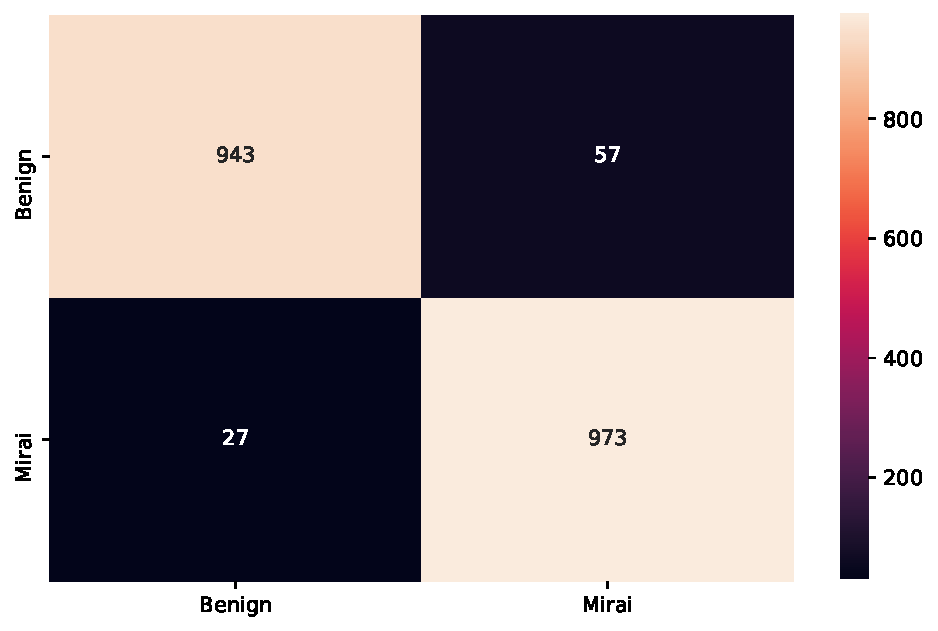
\includegraphics[width=.15\textwidth]{1.pdf}
	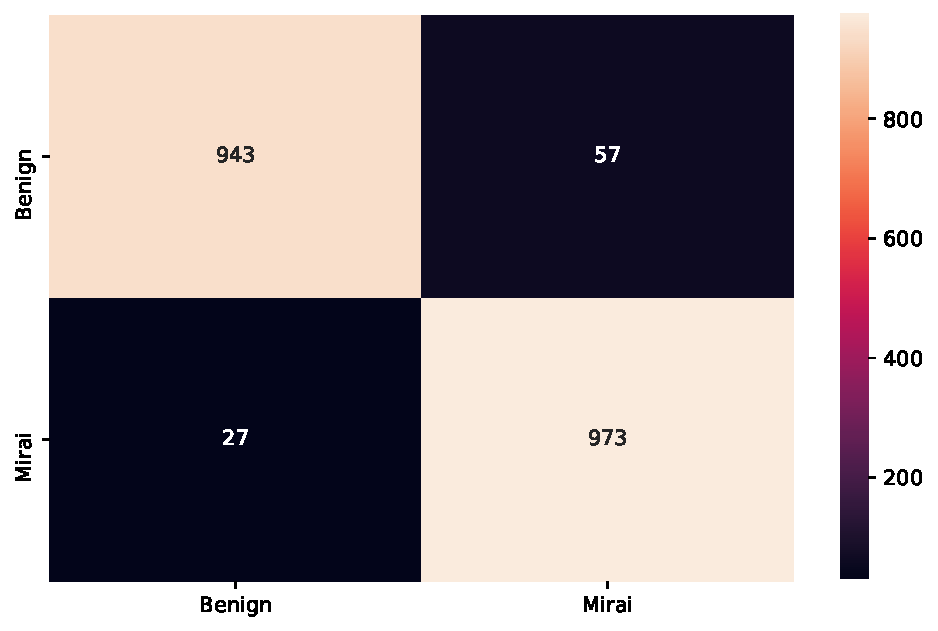
\includegraphics[width=.15\textwidth]{1.pdf}
	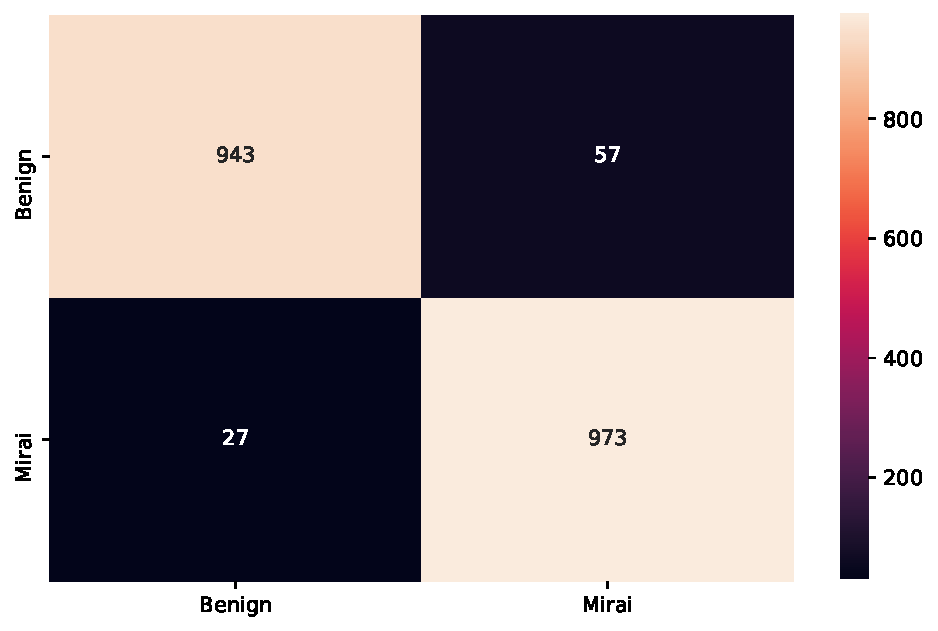
\includegraphics[width=.15\textwidth]{1.pdf}
	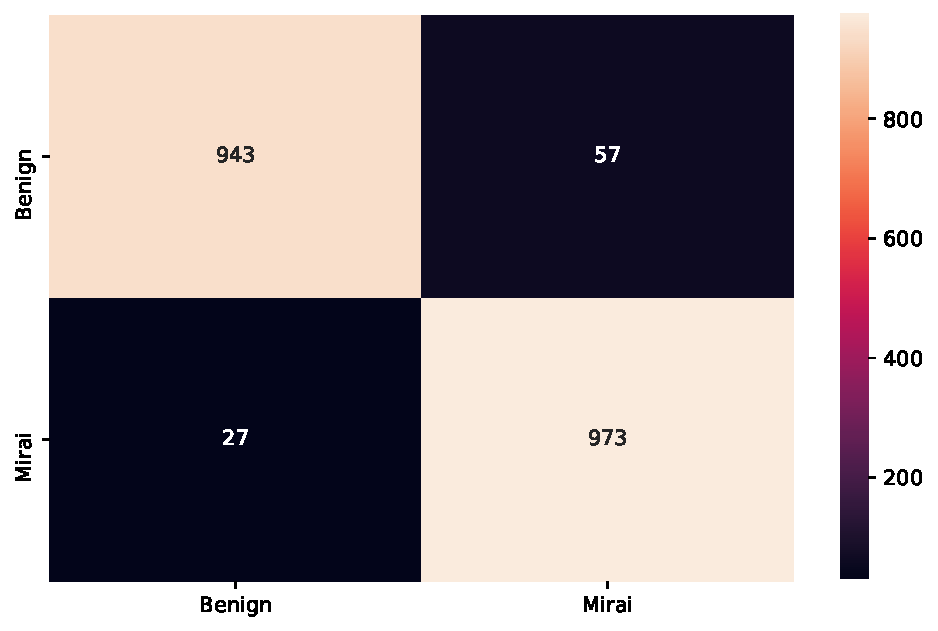
\includegraphics[width=.15\textwidth]{1.pdf}
	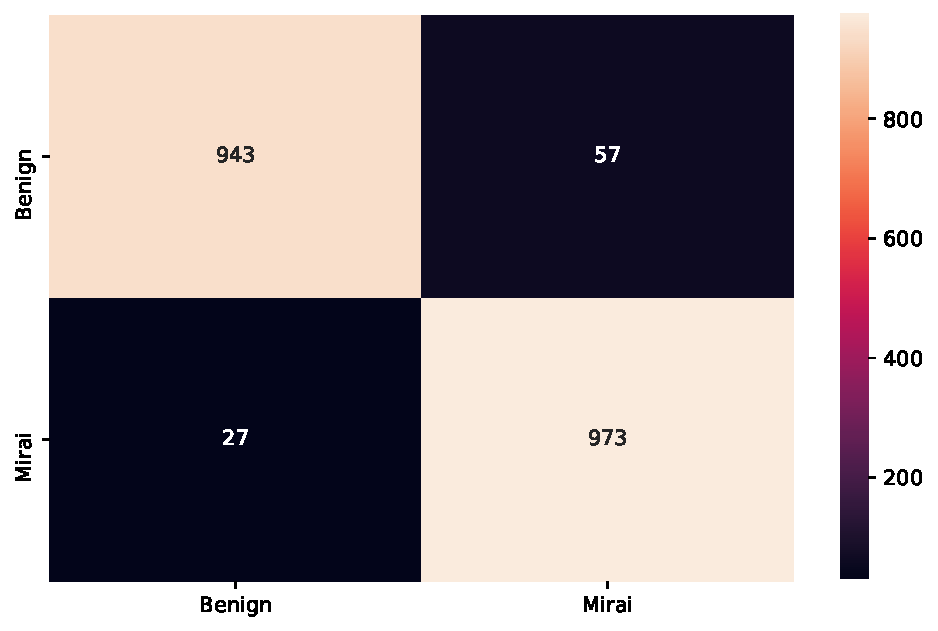
\includegraphics[width=.15\textwidth]{1.pdf}	
	\caption{default}
	\label{fig:figure3}
	
\end{figure}


\begin{figure}[htp]
	
	\centering
	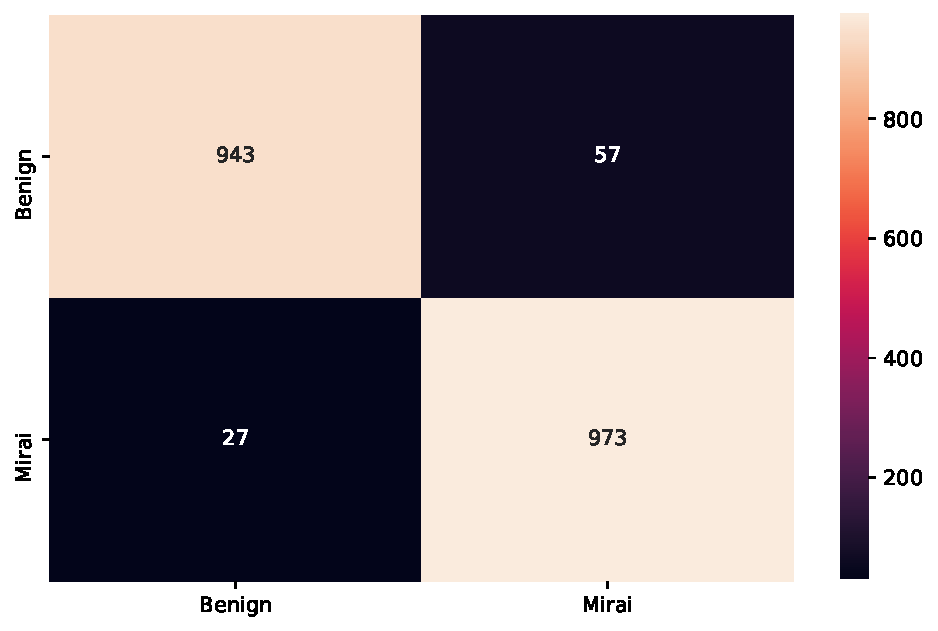
\includegraphics[width=.3\textwidth]{1.pdf}
	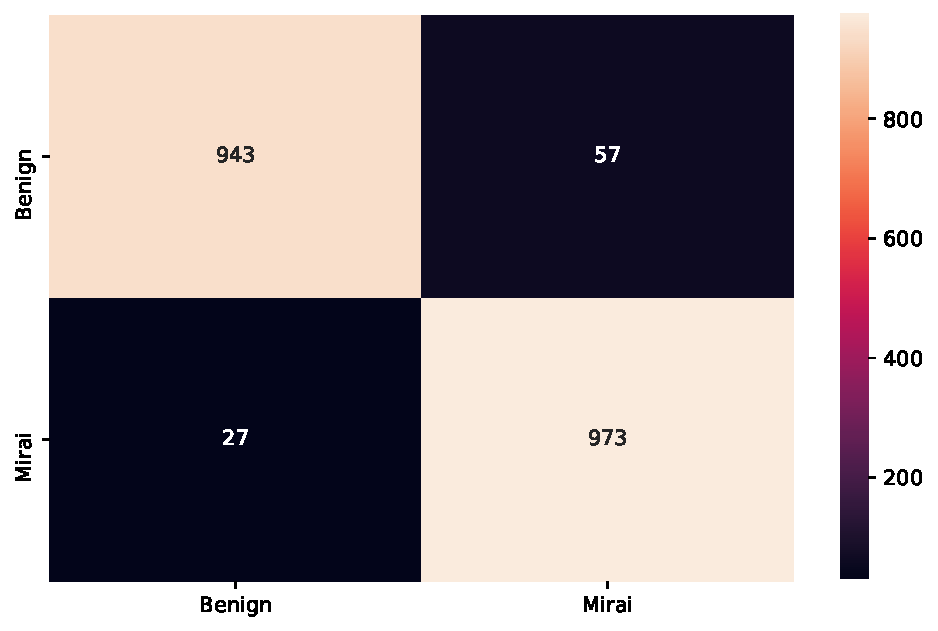
\includegraphics[width=.3\textwidth]{1.pdf}
	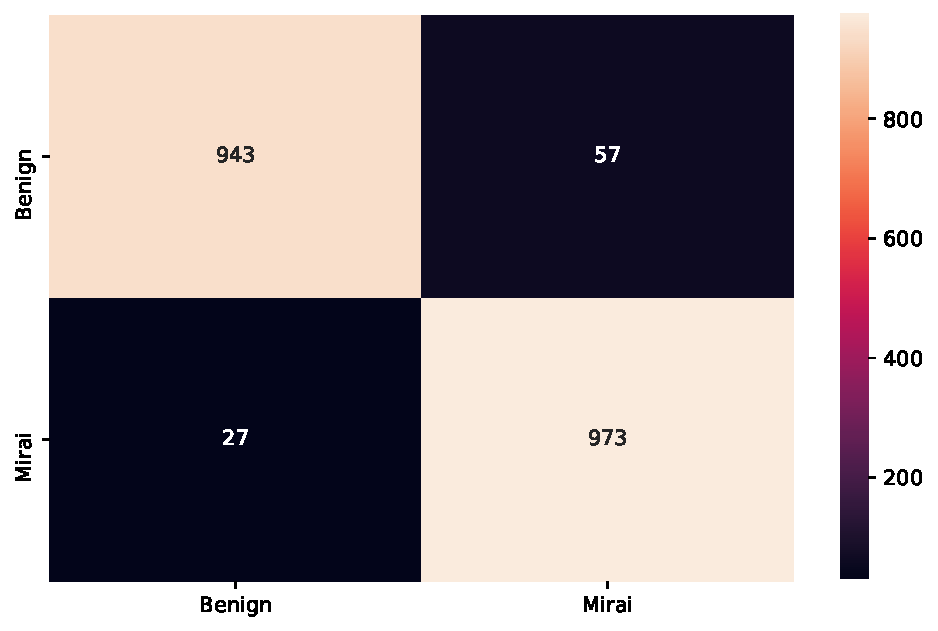
\includegraphics[width=.3\textwidth]{1.pdf}
	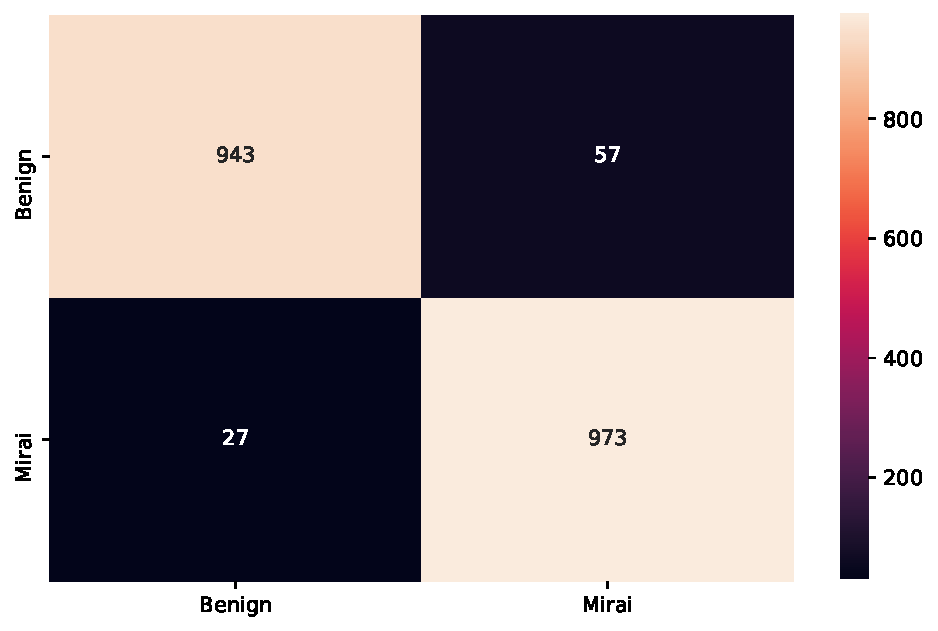
\includegraphics[width=.3\textwidth]{1.pdf}
	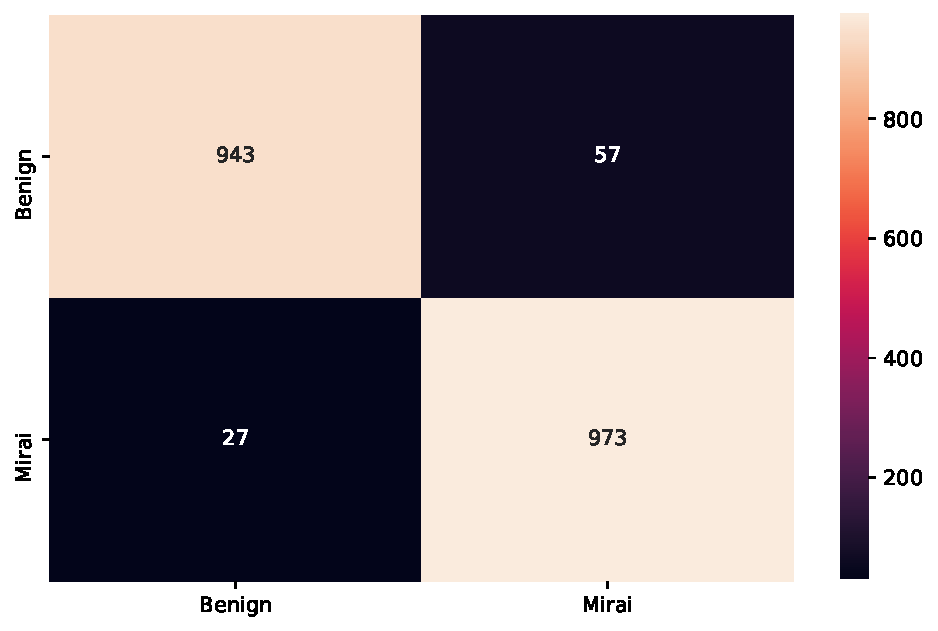
\includegraphics[width=.3\textwidth]{1.pdf}
	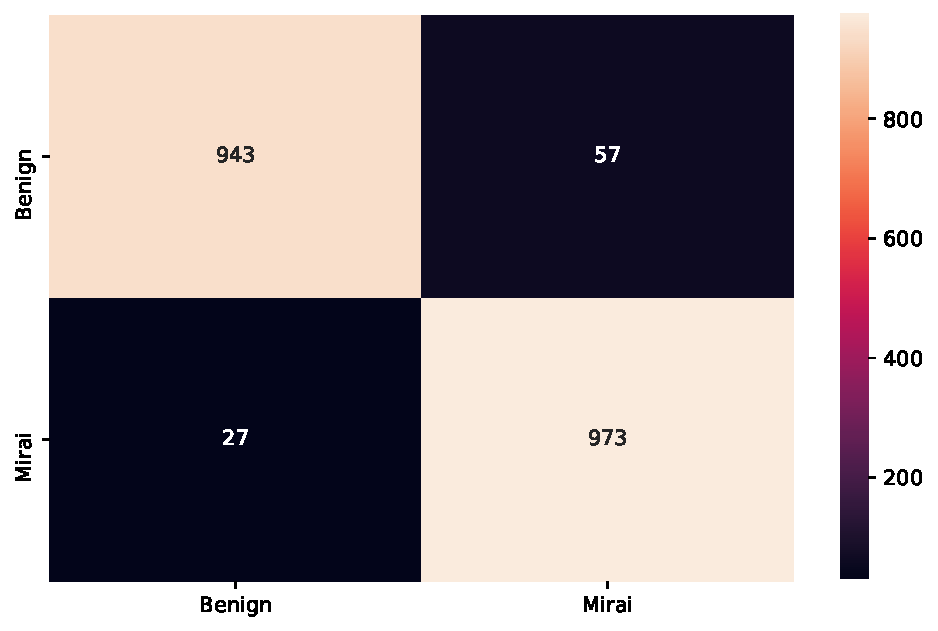
\includegraphics[width=.3\textwidth]{1.pdf}	
	\caption{default}
	\label{fig:figure3}
	
\end{figure}
\end{document}